\documentclass[preprint, 3p,
authoryear]{elsarticle} %review=doublespace preprint=single 5p=2 column
%%% Begin My package additions %%%%%%%%%%%%%%%%%%%

\usepackage[hyphens]{url}

  \journal{Energy Economics} % Sets Journal name

\usepackage{graphicx}
%%%%%%%%%%%%%%%% end my additions to header

\usepackage[T1]{fontenc}
\usepackage{lmodern}
\usepackage{amssymb,amsmath}
% TODO: Currently lineno needs to be loaded after amsmath because of conflict
% https://github.com/latex-lineno/lineno/issues/5
\usepackage{lineno} % add
\usepackage{ifxetex,ifluatex}
\usepackage{fixltx2e} % provides \textsubscript
% use upquote if available, for straight quotes in verbatim environments
\IfFileExists{upquote.sty}{\usepackage{upquote}}{}
\ifnum 0\ifxetex 1\fi\ifluatex 1\fi=0 % if pdftex
  \usepackage[utf8]{inputenc}
\else % if luatex or xelatex
  \usepackage{fontspec}
  \ifxetex
    \usepackage{xltxtra,xunicode}
  \fi
  \defaultfontfeatures{Mapping=tex-text,Scale=MatchLowercase}
  \newcommand{\euro}{€}
\fi
% use microtype if available
\IfFileExists{microtype.sty}{\usepackage{microtype}}{}
\usepackage[]{natbib}
\bibliographystyle{elsarticle-harv}

\ifxetex
  \usepackage[setpagesize=false, % page size defined by xetex
              unicode=false, % unicode breaks when used with xetex
              xetex]{hyperref}
\else
  \usepackage[unicode=true]{hyperref}
\fi
\hypersetup{breaklinks=true,
            bookmarks=true,
            pdfauthor={},
            pdftitle={European Carbon Market Connectedness and Risk Contagion: A Study of Return and Volatility Dynamics Between European Union Allowances (EUAs) and Financial Markets post-Fit for 55 and RePowerEU},
            colorlinks=false,
            urlcolor=blue,
            linkcolor=magenta,
            pdfborder={0 0 0}}

\setcounter{secnumdepth}{5}
% Pandoc toggle for numbering sections (defaults to be off)


% tightlist command for lists without linebreak
\providecommand{\tightlist}{%
  \setlength{\itemsep}{0pt}\setlength{\parskip}{0pt}}




\usepackage{subcaption}



\begin{document}


\begin{frontmatter}

  \title{European Carbon Market Connectedness and Risk Contagion: A
Study of Return and Volatility Dynamics Between European Union
Allowances (EUAs) and Financial Markets post-Fit for 55 and RePowerEU}
    \author[cisl,sigma]{Carlos Arcilla Barrera%
  %
  }
   \ead{ca577@cantab.ac.uk} 
    \author[cam]{Emre Usenmez%
  \corref{cor1}%
  }
   \ead{eu229@cam.ac.uk} 
      \affiliation[cisl]{
    organization={University of Cambridge Institute for Sustainability
Leadership},addressline={1 Regent Street},city={Cambridge},postcode={CB2
1GG},country={UK},}
    \affiliation[sigma]{
    organization={Sigma Advanced Capital Management},addressline={203
North LeSalle Dr, Suite
2110},city={Chicago},postcode={60601},country={USA},}
    \affiliation[cam]{
    organization={Gonville \& Caius College, University of
Cambridge},addressline={Trinity Street},city={Cambridge},postcode={CB2
1TA},country={UK},}
    \cortext[cor1]{Corresponding author}
  
  \begin{abstract}
  This paper uses Diebold-Yilmaz model to analyze the return and
  volatility connectedness between the European carbon market and the
  financial markets from the commencement of the 3rd phase of the EU
  emissions trading system in 2013 to August 2024 in order to ascertain
  the impact of both exogenous shocks and the recent reforms introduced
  under the Fit for 55 package and RePowerEU Plan. We examine the static
  and dynamic characteristics of the connectedness network and find that
  the return and volatility behavior of the European carbon market are
  primarily driven by their own fundamental factors, thus largely
  independent of other financial markets, except for coal and natural
  gas, and except during periods of financial stress where a relatively
  short-lived increase in the connectedness with other financial markets
  is observed.
  \end{abstract}
    \begin{keyword}
    Carbon markets \sep emissions trading system \sep connectedness
measures \sep 
    system risk
  \end{keyword}
  
 \end{frontmatter}

\hypertarget{introduction}{%
\section{Introduction}\label{introduction}}

In the late 19th century the Swedish scientist Svante Arrhenius
discovered\footnote{Building on the works of Joseph Fourier and John Tyndall roughly half a century earlier \citep{corfee-morlot_global_2007}}
the link between increases in carbon dioxide (CO2) concentrations in the
atmosphere, fossil fuel burning, and the greenhouse effect
\citep{corfee-morlot_global_2007, hart_scientific_1993, weart_discovery_2008}.
A century and a quarter later, in 2022, emissions worldwide have been
recorded at 57.4 gigatons of carbon dioxide equivalent (GtCO2e), with
the energy sector accounting for a little over third of these at 20.9
GtCO2e and industry another quarter at 14.4GtCO2e
\citep{unep_emissions_2023}.

As one of the top polluters \citep{unep_emissions_2023}, the European
Union (EU) has established an ambitious climate objective of 55\%
reduction in greenhouse gas emissions (GHGs) by 2030 from the 1990
levels \citep[Art 4(1)]{regulation_2021_1119}. To ensure the feasibility
of this objective, the European Commission (EC) has adopted a
comprehensive suite of legislative changes under Fit for 55 package
within a broader sustainable growth strategy under the European Green
Deal \citep{delivering_2021}.

In parallel to its decarbonization efforts, the EU also launched
RePowerEU Plan in 2022, a strategic response to the energy crisis
triggered by Russia's invasion of Ukraine in that year
\citep{communication_2022}. This plan aims to reduce the EU's dependency
on Russian fossil fuels by significantly accelerating the transition to
renewable energy sources, enhancing energy efficiency, and diversifying
the EU's energy supply chains \citep[1-5]{communication_2022}.

Under Fit for 55, the EC has proposed a set of reforms to the EU
emissions trading system (EU ETS) which have duly been adopted by the
European Commission in May 2023 \citep{directive_2023_959}. The EU ETS
itself is one of the central instruments of the EU in its
decarbonization and energy transition efforts
\citep{decision_2015_1814, bai_drivers_2023}, and it currently covers
about 40\% of the EU's GHG
emissions\footnote{The coverage will likely increase after the reforms are transposed into national laws of member states by 30 June 2024 \citep{directive_2023_959}}
\citep{eu_ets}. Under this mechanism a European Emission Allowance (EUA)
is a permit granting the right to emit one ton of CO2 which can then be
traded \citep{directive_2003_87}.

The EU ETS has evolved over four phases. The first phase, covering the
period from 2005 to 2007, has essentially established the market
mechanism underpinning the EU ETS \citep[Art. 11(1)]{directive_2003_87}.
The second phase, covering the five-year period from 1st of January
2008, has imposed a more stringent cap on the Union-wide total EUAs but
the mechanism still ended up with surplus of allowances largely due to
the 2008 recession \citep{ellerman_eu_2014, bel_emission_2015}. With the
commencement of the third phase on 1 January 2013, there has been a
shift from national allocation
plans\footnote{During the phases I and II of the EU emissions trading system (EU-ETS), each EU country decided on the allocation of their emission allowances. \citep[Art. 11]{directive_2003_87}}
to an EU-wide cap in the total number of
allowances\footnote{The total number of annual allowances also decrease by a linear factor of 1.74 percent. To address the surplus allowances that have been accumulating since Phase II, a new market stability reserve (MSR) has additionally been introduced that acts as a repository for excess portions of auctionable allowances and replenishes the market if allowances in circulation are fewer than 400 million \citep{decision_2015_1814, simoes_revision_2022}}
\citep[Art. 1]{directive_2009_29}. The fourth and current phase that
started in 2021, and will continue until 2030, has further reduced the
EU-wide allowance cap with more stringent rules for free
allocation\footnote{It also increased the annual reduction factor to 2.2 percent and earmarked a portion of MSR for innovation support.}
\citep{directive_2018_410}. In parallel, the Fit for 55 package has,
among other initiatives, extended the scope of the ETS to include
emissions from shipping and has accelerated the reduction of both the
free allocations and the total allowances within Phase
IV\footnote{This was done by increasing the linear reduction factor from 2.2 percent to 4.2 percent starting in 2024.}
\citep{directive_2023_959}.

The effectiveness of the EU ETS in decarbonizing and facilitating the
energy transition depends on several factors
\citep{backe_exploring_2023, de_cara_marginal_2011, marin_impact_2018, scheelhaase_options_2021}.
Among these factors, the price of EUAs plays a critical role
\citep{pietzcker_tightening_2021, quemin_raising_2022, lovcha_determinants_2022}.
Higher EUA prices have the potential to drive significant
transformations across multiple sectors, encouraging firms to innovate
and reduce emissions \citep{pietzcker_tightening_2021, recka_2015}. Such
realization of higher EUA prices can be aided by increased participation
of financial institutions which can promote liquidity, price discovery,
transparency, and improved market efficiency
\citep{bohl_impact_2023, corgnet_information_2021}. This in turn
depends, among other factors, on the price volatility which can raise
uncertainty and restrain investment into carbon-reducing technologies
\citep{acworth_emissions_2017, laing_assessing_2013}.

This study, therefore, analyzes, via return and volatility
connectedness, the degree of integration of EUAs with other asset
classes to assess potential diversification benefits EUAs may offer. If
present, such diversification benefits can consequently incentivize
increased participation by financial institutions and help the EU's
efforts in decarbonization and transitioning into renewables.
Accordingly, this study contributes to the literature on energy and
sustainable finance as well as on risk management in three complementary
ways. First, carbon is treated as an independent asset class whereas
previous works largely examine the issue within an energy context. To
the best of our knowledge, this is the first time it is treated as such
while incorporating the changes emerging from the Fit for 55 package and
RePowerEU. Within this context, this study considers return and
volatility spillovers within a broader range of markets, ranging from
fixed income and European and US equities to commodities. Second, while
the existing literature largely considers Phase III of EU ETS, this
study also incorporates Phase IV providing a more comprehensive analysis
of the recent changes. Third, market stress periods -- such as Covid-19
and the Russian-Ukrainian War -- are uniquely considered in analyzing
the changes in EU ETS connectedness and its integration with other asset
classes over time.

Three key results emerge from this study. First, we find that EUAs show
stronger connection with other financial markets mainly during periods
of financial crises. However, aside from connectedness with coal and
natural gas markets, these connections tend to be short-lived, and EUAs
generally remain independent. Second, our results indicate that the
European carbon market tend to be a net receiver of return and
volatility spillovers, suggesting that external factors influence this
market more than carbon-specific factors influence other markets. Third,
it appears that to date the reforms introduced by the Fit for 55
package, RePowerEU, and Phase IV may not have exerted as strong an
impact as market stresses, although it seems that their impact may have
a longer duration.

The rest of the paper is as follows. The next section provides a
literature review of the related studies. Section 3 specifies the
methodology and Section 4 describes the data. Section 5 presents the
main empirical findings and discussion, and Section 6 provides our
concluding remarks and implications.

\hypertarget{literature-review}{%
\section{Literature Review}\label{literature-review}}

Since the EU ETS has come into force, empirical literature on carbon
trading mechanisms has mainly focused on its price dynamics, on its
impact on the economy, and its relationship with various markets along
with its hedging benefits
\citep{demiralay_carbon_2022, dai_impact_2022}.

Ability to accurately forecast carbon prices are important in enabling
decisions on emissions and transition tradeoffs
\citep{wang_novel_2021, zhang_forecasting_2024, chen_multiscale_2024}.
To that end, while some have considered the role of attention in carbon
pricing
\citep{zheng_relationship_2022, gong_climate_2023, zhang_forecasting_2024},
some have used value-at-risk-forecasting, ARIMA, GARCH and its
modifications including, among others, Markov switching GARCH,
fractionality integrated GARCH, switching transition regression
exponential GARCH, and AR-GARCH to capture volatility, skewness, and
excess kurtosis
\citep{paolella_econometric_2008, benz_modeling_2009, arouri_nonlinearities_2012, byun_forecasting_2013, garcia-martos_modelling_2013, huang_hybrid_2021}.
Yet others have looked at the impact of policy uncertainties on the
volatility of carbon markets \citep{dai_impact_2022, dong_extreme_2024},
and some have used various decomposition and artificial intelligence
techniques to improve the forecasting ability
\citep{QIN2024131410, wang_novel_2021, chen_multiscale_2024}. What is
evident is that it is a challenge to forecast carbon prices since they
are nonstationary and show nonlinearity, and it is likely that the
information shocks transmit between different markets
\citep{feng_carbon_2011, lutz_nonlinearity_2013, segnon_modeling_2017, chen_multiscale_2024}.

Emissions trading can help in reducing the abatement costs and dampen
the negative impact of emission reductions on GDP
\citep{wu_achieving_2016, lin_impacts_2019}, although some of the carbon
reduction gains may decline overtime due to macroeconomic carbon rebound
effect \citep{bolat_is_2023}. Its impact on the economy, though, mainly
has a sectoral perspective. Within that perspective, the predominant
focus is on its strong impact on the energy industry
\citep{delarue_simulating_2007, kara_impacts_2008, zachmann_first_2008, kirat_impact_2011, bonenti_evaluating_2013, hobbie_windfall_2019, hanif_nonlinear_2021, dai_impact_2022},
and, to a lesser extent, on its negligible impact on the aviation,
cement, steel, and aluminum sectors
\citep{VANASSELT2007497, zhang_overview_2010, oberndorfer_costs_2007, efthymiou_eu_2019}.

There also appears to be a positive relationship, albeit in varying
degrees, between carbon markets on the one hand and equities, oil,
natural gas, coal, and electricity prices on the other
\citep{mansanet-bataller_co_2007, alberola_price_2008, keppler_causalities_2010, bredin_emerging_2011, chevallier_evaluating_2011, creti_carbon_2012, aatola_price_2013, zhang_dynamic_2016, ji_information_2018}.
However, with the changes introduced in each of the subsequent phases
such impacts became harder to establish
\citep{arouri_nonlinearities_2012, wu_market-linkage_2020}.
Nevertheless, there is likely a stronger relationship between carbon and
energy assets compared to financial assets for the duration of Phase II
and most of Phase III, which, for a non-energy portfolio, may provide
some diversification benefits
\citep{tan_how_2020, lovcha_determinants_2022, yang_idiosyncratic_2022}.
Moreover, interconnectedness of the carbon with other markets evolves
overtime and has increased with financial markets in recent years
\citep{jimenez-rodriguez_what_2019, tan_how_2020, dong_risk_2024}.
Concerning the integration of EUAs into portfolios, it seems to be the
case that incorporating a portion of carbon into stock portfolio
enhances the risk-adjusted performance of the portfolio
\citep{demiralay_carbon_2022}.

Even though many recent studies have offered some approaches to
understanding the linkage of EUAs with energy and other financial
markets, this study aims to expand that understanding further by
including the data that captures Phase IV of EU-ETS to date with a view
to examine the impacts of Fit for 55 reforms and the RePowerEU
initiative as well as the exogenous shocks such as COVID-19 and the
Russia-Ukraine war to those linkages. To this end, we hypothesize that
the reforms of Phase IV would maintain the potential diversification
benefits of carbon for a non-energy portfolio. That is, we hypothesize
that Phase IV reforms would not strongly alter the previous findings for
Phases II and III that carbon is linked more with energy assets than
financial assets. We also hypothesize that the impact of Fit for 55
reforms and RePowerEU Plan may strengthen the linkages with energy
markets since the former brings shipping emissions within its scope and
the latter aims to accelerate energy transition. Thus, we expect the
impact of these to be long lasting. On the other hand, we hypothesize
that the exogenous shocks would generate, or strengthen, short-lived
linkages with financial markets, though, as previous findings indicate,
shocks are likely to transmit between markets. We employ the following
methodology to test these hypotheses.

\hypertarget{methodology}{%
\section{Methodology}\label{methodology}}

The DY connectedness model proposed by
\citet{diebold_measuring_2009, diebold_better_2012, diebold_network_2014}
is a commonly employed method to evaluate the strength of relationships
among variables
\citep{zhang_dynamic_2016, xia_asymmetric_2019, ji_information_2019, tan_how_2020, gabauer_dynamic_2021, hanif_nonlinear_2021, diebold_past_2023, dong_risk_2024, gong_physical_2024}.
This approach allows us to assess the extent to which EUAs are linked to
other asset classes by examining the connectedness and transmission of
return and volatility shocks between markets and by exploring any
temporal changes to this relationship.

DY framework incorporates the forecast error variance decomposition
(FEVD) technique to measure both the overall and directional spillover
effects. It also introduces three primary time-varying spillover
measures: Total, Directional, and Pairwise Spillovers. This approach is
then further expanded by the Pairwise Connectedness Index (PCI), that
enables the quantification of spillover effects' strength between
specific pair of assets \citep{gabauer_dynamic_2021}.

Consider a variance stationary \(n\)-variable, \(VAR(p)\)
\begin{equation}
x_t = \sum_{i=1}^p\psi_ix_{t-i}+u_t
\end{equation} with the error term \(u_t \sim N(0,S_t)\) with \(S_t\)
denoting its variance-covariance matrices, and where \(x_t\) is an
\(n \times 1\) vector of endogenous variables, such as EUA daily returns
or volatility, \(\psi_i\) represents the autoregressive \(n \times n\)
matrices of the coefficients, and \(p\) is the length of lag with the
optimal lag length determined by the Bayesian information criterion
(BIC) \citep{diebold_better_2012, pham_impact_2023}.

Here, the moving average is represented using Wold's representation
theorem \citep{wold_study_1939} which decomposes every covariance
stationary process into two uncorrelated component process. If the
process is nondeterministic, then \begin{equation}
x_t = \sum_{j=0}^\infty A_ju_{t-j}
\end{equation} where \(A_j = \psi_1A_{i-1}+\psi_2A{i-2}+\dots\), with
\(A_j=0\) for \(j<0\), and \(A_0\) being an \(n \times n\) identity
matrix.

To solve the problem of orthogonal innovation,
\citet{diebold_better_2012} uses the generalized VAR framework proposed
by \citet{koop_impulse_1996} and \citet{pesaran_generalized_1998},
hereinafter referred to as KPPS. This framework produces variance
decompositions whereby they are invariant to the ordering. We can then
define fractions of the H-step-ahead error variances in forecasting
\(x_i\) into separate parts that are due to various system shocks. Those
fractions that are due to shocks to \(x_i\) , for \(i=1,2,\dots,n\), can
be referred to as own variance shares, and those that are due to shocks
to \(x_j\), \(j=1,2,\dots,n\) and \(i\neq j\), can be referred to as
cross-variance shares, or spillovers
\citep{diebold_better_2012, yang_idiosyncratic_2022, tan_how_2020, susilo_covid-19_2022}.

From the moving average representation, the generalized forecast error
variance decomposition (GFEVD) is then expressed as \begin{equation}
\theta_{ij}^g(H) = \frac{1}{\sigma_{jj}} \frac{\displaystyle\sum_{h=0}^{H-1}(e_i^TA_hS_te_j)^2}{\displaystyle\sum_{h=0}^{H-1}(e_i^TA_hS_tA_h^Te_i)}
\end{equation} where \(\sigma_{jj}\) standard deviation of the error
term of variable \(j\), \(e_i\) is the \(n \times 1\) selection vector
that takes on a value of one for \(i^{th}\) element and zero otherwise.
The index of spillover from variable \(j\) to variable \(i\) is
subsequently obtained by normalizing GFEVD by the row sum:
\begin{equation}
\tilde{\theta}_{ij}^g(H) = \frac{\theta_{ij}^g(H)}{\displaystyle\sum_{j=1}^n\theta_{ij}^g(H)}
\end{equation} where \(\tilde{\theta}_{ij}^g(H)\) is the percent of
forecast error in variable \(i\) that is explained by variable \(j\),and
by construction \(\sum_{j=1}^n\tilde{\theta}_{ij}^g(H) = 1\), and
\(\sum_{i,j=1}^n\tilde{\theta}_{ij}^g(H) = n\).

From this normalized GFEVD, we can obtain various connectedness indexes
which would in turn help summarize the overall connectedness within a
system's variables. Specifically, we can capture from all other markets
\(j\) within a system the total spillovers to market \(i\) with
\begin{align}
DSF_{n,i}(H) 
&= \frac{\displaystyle\sum_{j=1,i\neq j}^n\tilde{\theta}_{ij}^g(H)}{\displaystyle\sum_{i,j=1}^n\tilde{\theta}_{ij}^g(H)} \times 100 \\
&= \frac{100}{n}\sum_{i=1, i\neq j}^n\tilde{\theta}_{ij}^g(H)
\end{align} with a high measure indicating that variable \(i\) is highly
responsive to shocks from other markets. Similarly, the total spillovers
from variable \(i\) to all other variables, can be captured with
\begin{equation}
DST_{n,i}(H) = \frac{100}{n}\sum_{j=1,i \neq j}^n \tilde{\theta}_{ij}^g(H).
\end{equation} The net directional spillover (NS) from \(i\) to \(j\)
results from the difference between the directional spillovers DST and
DSF and represents the net contribution of a specific market to the
others. A positive NS indicates that market \(i\) is a net shock
transmitter. This means, the impact market \(i\) has on all other
markets \(j\) is larger than the impacts of all other markets \(j\) has
on market \(i\). A negative NS, on the other hand, indicates that market
\(i\) is a net shock receiver. Thus, the net directional spillover is
calculated as \begin{equation}
NS_{n,i}(H) = DST_{n,i}(H) - DSF_{n,i}(H).
\end{equation} Although the NS provides important information on how
much of volatility in other markets are attributable to each market in
net terms, it is also important to be able to capture the overall degree
of connection between two markets. This is then captured by the net
pairwise directional spillover (NPDS) index, defined as the difference
between the gross shocks transmitted from variable \(i\) to variable
\(j\) \citet{diebold_better_2012}: \begin{equation}
NPDS_{ij}(H)=\frac{100}{n}(\tilde{\theta}_{ij}^g(H) - \tilde{\theta}_{ji}^g(H)).
\end{equation} The volatility spillover or total connectedness index
(TCI) and their equivalences are then constructed as \begin{align}
TCI(H) 
&= \frac{\displaystyle\sum_{j=1, i\neq j}^n\tilde{\theta}_{ij}^g(H)}{\displaystyle\sum_{i,j=1}^n\tilde{\theta}_{ij}^g(H)} \times 100 \\
&= \frac{100}{n}\sum_{j=1, i \neq j}^n\tilde{\theta}_{ij}^g(H) = \frac{1}{n}\sum_{j=1}^nDSF_{n,i}(H) = \frac{1}{n}\sum_{i=1}^nDST_{n,i}(H). 
\end{align} In line with \citet{gabauer_dynamic_2021}, we use the Pair
Connectedness Index (PCI) that captures the overall degree of connection
between two markets. When considering a network with only two series,
the PCI and TCI are equivalent. However, TCI calculation between two
series may yield a biased result because by design the approach
considers only two series despite each series may be impacted by more
series. PCI computation based on a large network, on the other hand, is
not only more efficient than calculating the TCI of multiple small
networks, but also yields a more accurate result due to the unbiased
coefficient estimates of the VAR model. It is calculated as follows:
\begin{equation}
PCI_{ij} = 2 \times \frac{\tilde{\theta}_{ij}^g(H) + \tilde{\theta}_{ji}^g(H)}{\tilde{\theta}_{ij}^g(H)+\tilde{\theta}_{ji}^g(H)+\tilde{\theta}_{jj}^g(H)+\tilde{\theta}_{ii}^g(H)}
\end{equation} The PCI ranges between \(0\) and \(1\) illustrating the
overall degree of bilateral interconnectedness across two variables
\(i\) and \(j\).

\hypertarget{data}{%
\section{Data}\label{data}}

We obtain daily price data for EUAs and other financial markets from
Bloomberg LP and Refinitiv, covering the period from January 2, 2013, to
August 16, 2024. This time frame, as shown in Figure \ref{fig:EUAprice},
encompasses Phases III and, to the extent possible, Phase IV of the
European Union Emissions Trading System (EU ETS), including the reforms
introduced under Fit for 55 package and RePowerEU. It also includes key
economic periods characterized by significant market volatility, such as
the 2016 Brexit referendum, the COVID-19 pandemic especially between
February and April 2020, and the escalation of the Russian-Ukrainian
conflict in March-April 2022.

\begin{figure}[htpb]
\caption{European Emission Trading System Phases and European Union Allowances (EUA) Prices}
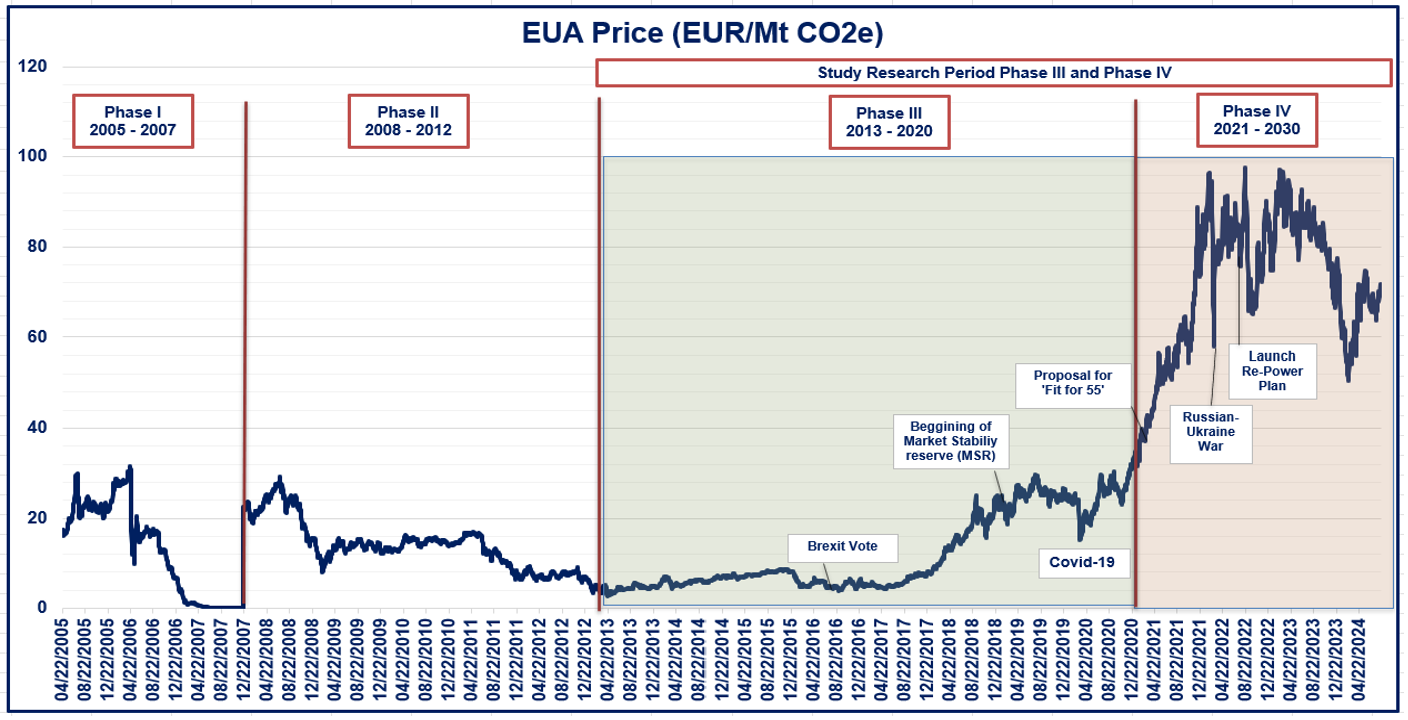
\includegraphics[width = \textwidth]{../figures/1-EUAPrice}
\label{fig:EUAprice}
\end{figure}

For the same period, we also obtain price data for Stoxx 600 Index as a
proxy for the European equity market and the S\&P 500 Index as a proxy
for the International Equity Index. For European sovereign bond markets
we utilize iBoxx Eurozone Sovereign Performance Index, and for European
corporate bond markets we use iBoxx Eur Corporates Index as proxies. To
represent the commodity markets, we additionally obtain the Bloomberg
Metal Commodity Index and the Bloomberg Commodity ex Energy Index, as
energy market exposure is captured separately.

The EUA is represented by the continuous contracts of the most actively
traded financial futures. Given the carbon markets intrinsic
relationship with energy markets, the latter are analyzed independently.
Specifically, we use continuous futures contracts for Brent crude oil,
API2 Rotterdam coal, and TTF natural gas as proxies for the Europeal
oil, coal, and gas markets, respectively. In total, this data set
comprises of 30,140 observations. All prices are converted to EUR to
eliminate the impact of currency fluctuations. Returns are
log-normalized, and volatilities are estimated based on a rolling window
of 20-day daily returns.

Table \ref{table:descriptivestats} provides the descriptive statistics
of daily returns in panel (a) and volatility in panel (b). Both panels
show that all variables are skewed and leptokurtic. Together with
Jarque-Bera that strongly rejects the null hypothesis of a normal
distribution, it is evident that none of the variables conform to a
normal distribution.\\

\begin{table}[htpb]
  \caption{Descriptive statistics of daily return and volatility}
  \bigskip
  \label{table:descriptivestats}
    \begin{tabular}{|l|l|l|l|l|l|l|l|l|l|l|} 
    \multicolumn{11}{@{}l}{\em(a) Daily logarithmic return}\\ \hline
          & Mean & Median & Max & Min & St.Dev. & Skewness & Kurtosis & Obs. & J-B & Prob. \\ \hline
        CARBON & 0.0013 & 0.0008 & 0.2690 & -0.3508 & 0.0311 & -0.2896 & 10.6147 & 3011 & 14177.78 & 0 \\ \hline
        EUROSTOXX & 0.0003 & 0.0006 & 0.0840 & -0.1148 & 0.0099 & -0.8462 & 11.3898 & 3011 & 16634.71 & 0 \\ \hline
        BRENTOIL & 0.0002 & 0.0008 & 0.2224 & -0.2483 & 0.0230 & -0.1878 & 14.1649 & 3011 & 25190.26 & 0 \\ \hline
        COALAPI & 0.0005 & 0.0000 & 0.5935 & -0.2571 & 0.0274 & 3.2819 & 98.0915 & 3011 & 1212557 & 0 \\ \hline
        NATGAS & 0.0009 & -0.0001 & 0.5034 & -0.2983 & 0.0401 & 1.2270 & 17.3396 & 3011 & 38475.98 & 0 \\ \hline
        EURSOVER & 0.0001 & 0.0001 & 0.0200 & -0.0171 & 0.0030 & 0.1270 & 4.3384 & 3011 & 2369.475 & 0 \\ \hline
        EURCORP & 0.0001 & 0.0001 & 0.0137 & -0.0218 & 0.0019 & -0.6075 & 12.0755 & 3011 & 18479.1 & 0 \\ \hline
        SPXINDEX & 0.0006 & 0.0006 & 0.1032 & -0.1260 & 0.0114 & -0.4644 & 13.8660 & 3011 & 24229.62 & 0 \\ \hline
        COMEXENG & 0.0000 & 0.0000 & 0.0407 & -0.0396 & 0.0072 & -0.0775 & 2.1079 & 3011 & 560.4679 & 0 \\ \hline
        METALS & 0.0001 & 0.0000 & 0.0599 & -0.0969 & 0.0101 & -0.3869 & 6.4988 & 3011 & 5373.834 & 0 \\ \hline
  
    \end{tabular}
    
\bigskip
    \begin{tabular}{|l|l|l|l|l|l|l|l|l|l|l|} 
    \multicolumn{11}{@{}l}{\em(b) Volatility}\\ \hline
          & Mean & Median & Max & Min & St.Dev. & Skewness & Kurtosis & Obs & J-B & Prob. \\ \hline
        CARBON & 0.4402 & 0.3916 & 1.8455 & 0.1317 & 0.2265 & 2.2435 & 7.7022 & 3014 & 9978.411 & 0 \\ \hline
        EUROSTOXX & 0.1383 & 0.1223 & 0.7035 & 0.0315 & 0.0753 & 2.8685 & 13.9645 & 3014 & 28623.02 & 0 \\ \hline
        BRENTOIL & 0.3151 & 0.2732 & 1.6611 & 0.0772 & 0.1852 & 2.7509 & 10.9659 & 3014 & 18903 & 0 \\ \hline
        COALAPI & 0.3135 & 0.2241 & 2.6857 & 0.0000 & 0.2985 & 3.7413 & 20.9101 & 3014 & 61940.62 & 0 \\ \hline
        NATGAS & 0.4863 & 0.3490 & 3.1750 & 0.0506 & 0.4070 & 2.2835 & 8.3829 & 3014 & 11444.49 & 0 \\ \hline
        EURSOVER & 0.0422 & 0.0354 & 0.1337 & 0.0129 & 0.0223 & 1.5943 & 2.5774 & 3014 & 2111.037 & 0 \\ \hline
        EURCORP & 0.0248 & 0.0189 & 0.1130 & 0.0071 & 0.0154 & 2.1823 & 5.9139 & 3014 & 6784.517 & 0 \\ \hline
        SPXINDEX & 0.1546 & 0.1306 & 1.0152 & 0.0574 & 0.0942 & 4.7283 & 34.8012 & 3014 & 163327.9 & 0 \\ \hline
        COMEXENG & 0.1080 & 0.1010 & 0.3428 & 0.0460 & 0.0373 & 2.1601 & 7.9794 & 3014 & 10339.95 & 0 \\ \hline
        METALS & 0.1476 & 0.1343 & 0.4863 & 0.0482 & 0.0624 & 1.7810 & 4.8952 & 3014 & 4602.693 & 0 \\ \hline
    \end{tabular}
\end{table}

Following previous studies
\citep{diebold_better_2012, reboredo_volatility_2014, gabauer_dynamic_2021}
we transform the data with logarithmic returns and 20-day volatility of
logarithmic returns.

For connectedness analysis, it is also essential that the time series
data are stationary \citep{diebold_better_2012, zhang_oil_2017}. To test
for stationarity, we employ Augmented Dickey-Fuller (ADF)
\citep{dickey_distribution_1979} and Phillips-Perron (PP)
\citep{phillips_testing_1988} tests. Both tests strongly reject the null
hypothesis for a presence of a unit root in either returns (p = 0.000)
or volatility data (p=0.000), suggesting that they are both stationary.

\bibliography{EUAbibliography.bib}


\end{document}
